\documentclass[a4paper,11pt]{article} \usepackage[T1]{fontenc} \usepackage[utf8]{inputenc} \usepackage[francais]{babel}
\usepackage[top=2cm,left=2.5cm,right=2.5cm,bottom=2cm]{geometry} % Géométrie de la page, modifier selon le besoin
\usepackage{xcolor, listingsutf8, textcomp, float, lmodern, wrapfig, textcomp, tikz, graphicx}
\usepackage[colorlinks=true,citecolor=black,linkcolor=black, urlcolor=blue]{hyperref}

\lstset{language=C++, keywordstyle=\bfseries\ttfamily\color[rgb]{0,0,1}, identifierstyle=\ttfamily, commentstyle=\color[rgb]{0.133,0.545,0.133},stringstyle=\ttfamily\color[rgb]{0.627,0.126,0.941}, showstringspaces=false, basicstyle=\small, tabsize=2, breaklines=true,prebreak=\raisebox{0ex}[0ex][0ex]{\ensuremath{\hookleftarrow}}, breakatwhitespace=false, aboveskip={\baselineskip}, columns=fixed,upquote=true, extendedchars=true, inputencoding=utf8/latin1}
\lstset{language=C++}

\begin{document}
  \begin{titlepage}
%
\includegraphics[scale=0.45]{Images/logo_phelma.pdf}\hfill
\begin{center}
    \vspace*{1cm}
    \textsc{\Large Bureau d'Études d'Informatique}\\
    [4.5cm] \rule{\linewidth}{0.5mm}\\[0.4cm]
    {\huge\bfseries Fractales et FLTK\\
    [0.4cm]}\rule{\linewidth}{0.5mm}\\[1.0cm]
    \textsc{pmpB}
    \begin{flushright} \large
        % \emph{Entrepreneurs :} \\
        Julia \textsc{Dupuis}\\
        Nils \textsc{Exibard}\\
        Félix \textsc{Piédallu}\\
    \end{flushright}
    
    
  \begin{center}
    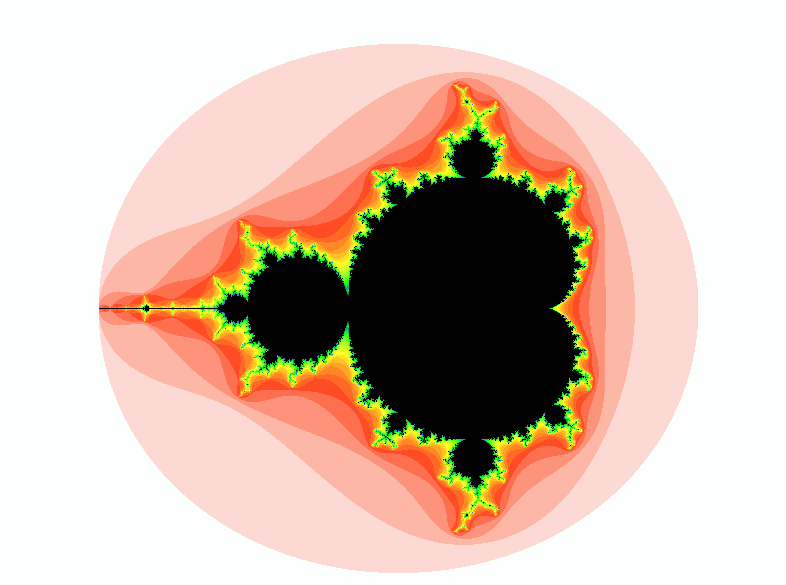
\includegraphics[width=0.7\textwidth]{Images/Titlepage.png}
  \end{center}

    \vfill

    \large{\today}
\end{center}
\end{titlepage}
     % Fichier de page de titre
  \pagenumbering{arabic}  % Pas de numérotation
  \tableofcontents          % Table des matières avec liens, générée automatiquement.
\vspace{3cm}
% On peut faire une nouvelle page avec  \newpage

\section{Présentation du logiciel - Notice d'utilisation}
Le sujet  sur lequel nous avons choisi de travailler est le projet « Fractales », grand classique de la programmation, utilisant le plan complexe.
\begin{figure}[H] \begin{center} 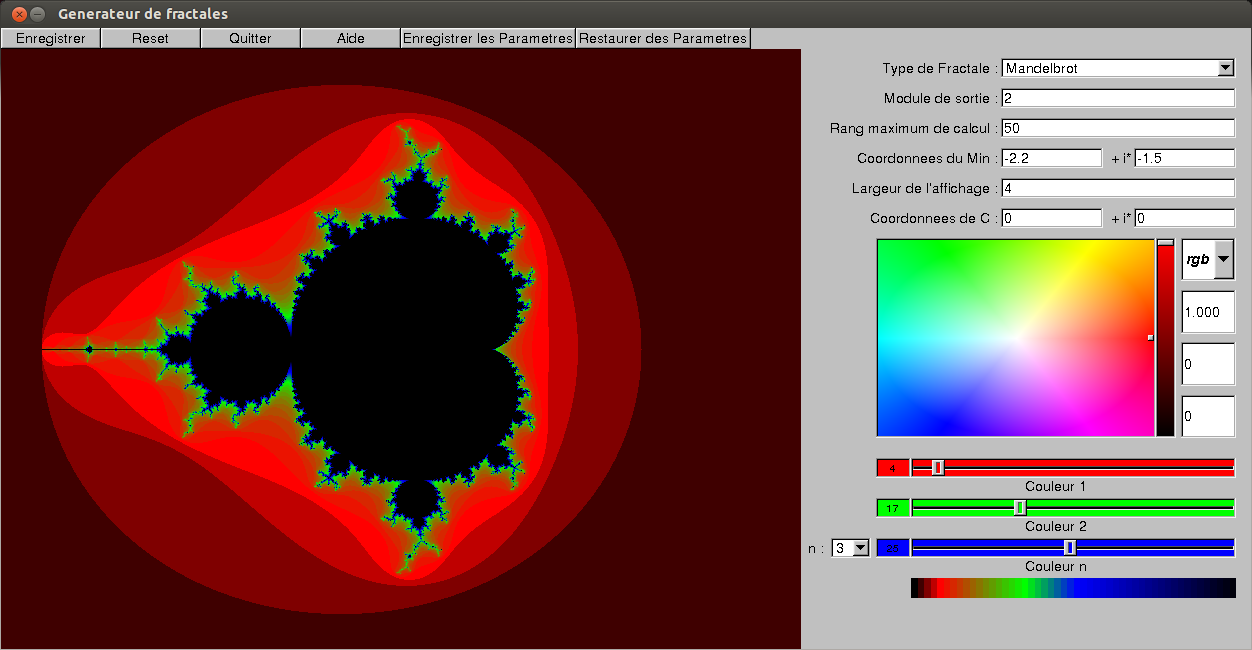
\includegraphics[width=\textwidth]{Images/InterfaceTotale.png}
    \caption{Aperçu du logiciel}
\end{center} \end{figure}

Ce logiciel permet d'afficher et d'explorer différents types de fractales, notamment les ensembles de Mandelbrot et de Julia. On peut se déplacer, zoomer, et choisir les couleurs du dégradé permettant un affichage intéressant de la fractale.\\

Le logiciel se veut assez intuitif pour qui connaît le vocabulaire des fractales, et ses  principales fonctions sont décrite ici :\\

\begin{itemize}
  \item Une section de l'interface permet de choisir les différents paramètres de calcul et d'affichage de la fractale (type, module de sortie, rang maximal, coordonnées du point inférieur gauche, largeur de l’affichage, coordonnées de la constante C utilisée par Julia)
        \begin{figure}[H] \begin{center} 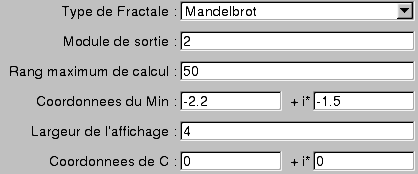
\includegraphics[width=0.5\textwidth]{Images/Parametres.png}
            \caption{Choix des paramètres généraux de la fractale}
        \end{center} \end{figure}


  \item Une autre permet la gestion des couleurs (jusqu'à 10 couleurs, avec écart modifiable selon le rang de divergence).
        \begin{figure}[H] \begin{center} 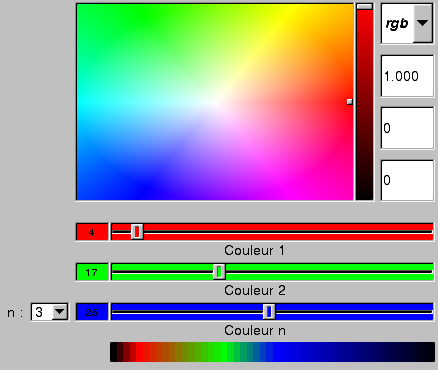
\includegraphics[width=0.5\textwidth]{Images/ChoixCouleurs.png}
            \caption{Choix de la couleur et des points de contrôle du dégradé}
        \end{center} \end{figure}
  \item On peut enregistrer l'image a résolution souhaitée, ou bien n'en enregistrer que les paramètres.
  \item Restaurez les paramètres précédemment enregistrés.
  \item Réinitialisez les paramètres (Bouton Reset).
  \item Fonction « Quitter ».
  \item Un bouton "Aide" donne les interactions possible avec la souris.
        \begin{figure}[H] \begin{center} 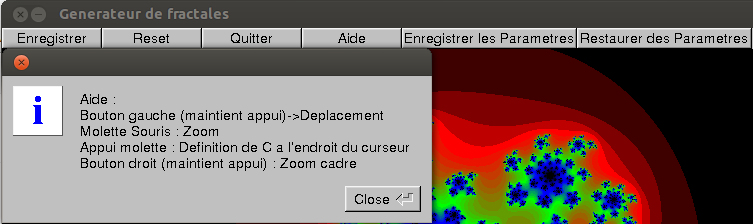
\includegraphics[width=0.8\textwidth]{Images/Aide.png}
            \caption{Petite aide}
        \end{center} \end{figure}
  \item Déplacer l’image avec le clic gauche maintenu.
  \item Zoom cadre (bouton droit) ou zoom centré sur la souris (molette).
        \begin{figure}[H] \begin{center} 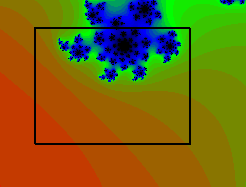
\includegraphics[width=0.5\textwidth]{Images/Cadre.png}
            \caption{Zoom cadre, en maintenant le bouton droit de la souris}
        \end{center} \end{figure}

\end{itemize}



\section{Sources - Notice de maintenance}

\subsection{Affichage}%à remplir

\subsection{Structures de données}
\begin{lstlisting}
struct Pixel {
    complex<double> z;      //Coordonnées du pixel dans le plan complexe
    int n;                  //Rang de divergence du pixel
};
\end{lstlisting}

Cette structure permettra de tracer la fractale à partir du rang de divergence et de la coordonnée de chaque pixel.

\begin{lstlisting}
struct Donnees {
    enum fractype Fractale; // Type de fractales choisie (Type énuméré)
    int     rangMax;        // Rang maximal de convergence
    double  moduleMax;      // Module de convergence (determination de la convergence on non de la fonction)
    complex<double> C;      // Constante de calcul
    complex<double> ig;     // Coordonnees du point inferieur gauche
    double pasxy;           // Pas de la matrice (incrementation, en fait, et egale dans les 2 dimensions, car pixels carres)
    struct Pixel Tab[L_ZONE][H_ZONE]; // Matrice des pixels de l'image.
int hauteur;             //Hauteur de l'image
    unsigned char buffer[3*L_ZONE*H_ZONE];//contient l'image sous forme RGB
    unsigned char bufferDeg[3*325];//contient l'apperçu du dégradé sous forme RGB
    int nbSlider;           //Nombre de slider actifs
    unsigned long int slider[MAX_SLIDER+2][2];//contient le rang et la couleur de chaque slider
};

\end{lstlisting}

Cette structure est la plus importante du programme.

\begin{lstlisting}
struct Tests {
    bool dessin;//faut-il refaire le dessin?
    bool calcul;//faut il refaire le calcul
    bool calccouleurs;//faut il refaire le calcul des couleurs ?
    int slider; //contient le slider actif
};\end{lstlisting}

Cette structure contient les variables nécessaires à la vérification des conditions, cela permet entre autre d’éviter les calculs inutiles.

\begin{lstlisting}
enum fractype {
    MANDELBROT,
    JULIA,
    COSC,
    SINZO,
    PERSONNA//Originellement prévue pour une fractale personnalisée, non utilisée faute de temps
};\end{lstlisting}

Le type énuméré permet d'utiliser plus facilement les différents types de fractales.\\

\subsection{Fonctions}
\begin{lstlisting}
void InitialiserDonnees(); \end{lstlisting}

Initialise les données du programmes

\begin{lstlisting}
void realFromTab(double *bi, double *bj);\end{lstlisting}

Effectue la correspondance entre les coordonnées complexe et les pixels

\begin{lstlisting}
pointeurFct retourne_fonction();\end{lstlisting}

Retourne la fonction de calcul de la fractale, pour son utilisation dans le projet. 

\begin{lstlisting}
int mandelbrot(complex<double> position);
int julia     (complex<double> position);
int sinzo     (complex<double> position);
int cosc      (complex<double> position);
int personna  (complex<double> position);\end{lstlisting}

Voici alors les fonctions fractales utilisées ; elles retournent un rang de convergence en un point du plan complexe.


\begin{lstlisting}
void convergenceLigne(int j, pointeurFct fonction);\end{lstlisting}

Etudie la convergence ligne par ligne

\begin{lstlisting}
void degradeRGB(unsigned long A, unsigned long B, int N, int tab[][3]);\end{lstlisting} 

Effectue le calcul d'un dégradé de taille N entre une couleur A et une couleur B, et stocke les trois composantes RGB dans tab

\begin{lstlisting}
void couleursRGB(unsigned long tabSlider[][2],int tab[][3]);\end{lstlisting}

Remplit tab d'une suite de dégradé grâce à degradeRGB à partir des informations contenues dans tabSlider

\begin{lstlisting}
void calcBuffer(int tabdeg[][3]);\end{lstlisting}

Calcule et stocke dans gDonnees.bufferDeg à partir d'un tableau de couleurs RGB

\begin{lstlisting}
int enregistrerPPM(int Largeur, char Fichier[32]);\end{lstlisting}

Enregistre une image en ppm de Largeur pixel de large et de ratio constant dans Fichier.

\begin{lstlisting}
void enregistrerParams(const char* fichier);
void restaurerParams(const char* fichier);\end{lstlisting}

Permet d'enregistrer (et de lire, mais non finalisé) les paramètres permettant de redessiner la fractale.\\

\subsection{Dessin}
\begin{lstlisting}
void ZoneDessinInitialisation(Fl_Widget* widget, void* data);\end{lstlisting}
%Initialise la zone de dessin puis appelle gestionAffichage_iter
\begin{lstlisting}
void afficheFractaleLigne();\end{lstlisting}

Commande le calcul puis l'affichage d'une ligne

\begin{lstlisting}
void afficheLigneRGB(int j, int tableauCouleurs[][3]);\end{lstlisting}

Affiche la ligne j avec pour couleurs un tableau RGB

\begin{lstlisting}
void gestionAffichage_iter(void* data);//iter car en remplacement de la fonction recursive d'origine.\end{lstlisting}

Calcule \emph{SI nécessaire} la fractale puis l'affiche grâce aux diverses autres fonctions.

\begin{lstlisting}
void tracerCadre (int x1, int y1 , int x2, int y2);\end{lstlisting}

Trace le cadre du zoom cadre a partir de 2 points (conserve le ratio d'écran)

\begin{lstlisting}
void zoneDegrade(Fl_Widget* widget, void* data);\end{lstlisting}

Gère l'affichage de la zone d’aperçu du dégradé.\\

\subsection{Callback}
\begin{lstlisting}
void ZoneDessinSourisCB (Fl_Widget* widget, void* data ) ;\end{lstlisting}

Gère l'ensemble des événements commandables à l'aide de la souris, à savoir le zoom molette, le zoom cadre(clic droit), le déplacement de l'affichage(clic gauche) et choix de la constante (clic molette)

\begin{lstlisting}
void ChampModuleDeSortieCB(Fl_Widget* w, void* data);\end{lstlisting}

Permet de régler le module de sortie de la fractale (module à partir duquel on considère qu'il y a convergence)

\begin{lstlisting}
void ChampProfondeurCB  (Fl_Widget* w, void* data);\end{lstlisting}

Choix du rang maximal d'étude

\begin{lstlisting}
void MenuFractaleCB     (Fl_Widget* w, void* data);\end{lstlisting}

Met en relation la fractale choisie par l'utilisateur avec sa fonction de calcul.\\

Voici les différents boutons de la barre de menu :
\begin{lstlisting}
void BoutonQuitterCB    (Fl_Widget* w, void* data);\end{lstlisting}

\begin{lstlisting}
void BoutonEnregistrerCB(Fl_Widget* w, void* data);\end{lstlisting}

\begin{lstlisting}
void BoutonResetCB      (Fl_Widget* w, void* data);\end{lstlisting}

\begin{lstlisting}
void BoutonAideCB       (Fl_Widget* w, void* data);\end{lstlisting}

\begin{lstlisting}
void BoutonSaveParamsCB (Fl_Widget* w, void* data);\end{lstlisting}

Permet de sauvegarder les paramètres actuels.

\begin{lstlisting}
void BoutonBackParamsCB (Fl_Widget* w, void* data);\end{lstlisting}

Permet de revenir aux paramètres précédemment sauvegardés.

\begin{lstlisting}
void ChampXMinCB        (Fl_Widget* w, void* data);
void ChampYMinCB        (Fl_Widget* w, void* data);
void ChampLargeurCB     (Fl_Widget* w, void* data);\end{lstlisting}

Définit le point inférieur gauche et la largeur de l'affichage ( taille en complexe)

\begin{lstlisting}
void ChampCXCB          (Fl_Widget* w, void* data);
void ChampCYCB          (Fl_Widget* w, void* data);\end{lstlisting}

Permet de rentrer une valeur de constante (utilisée dans certaines fractales)

\begin{lstlisting}
void CarreChoixCouleurCB(Fl_Widget* w, void* data);
void Slider1CB          (Fl_Widget* w, void* data);
void Slider2CB          (Fl_Widget* w, void* data);
void ChoixSliderCB		(Fl_Widget* w, void* data);
void Slider3CB          (Fl_Widget* w, void* data);\end{lstlisting}

Ces trois callbacks permettent la gestion des couleurs

\begin{lstlisting}
void setColorChooserColor(unsigned long int couleur);\end{lstlisting}~\\

\section{Critique}

%En vrac, à retravailler mais l'idée est la : 
\begin{itemize}
  \item La fonction d'affichage est chaotique, elle appelle d'abord "initialiser\_affichage" qui appelle elle même "gestionAffichage\_iter".% Si je me souviens bien ça évitait un bug fut un temps, Félix, je te laisse en parler.

  \item La structure de données initiale pour les couleurs, qui limitaient le programme à 3 sliders. Il a fallu réécrire beaucoup de choses pour pouvoir augmenter le nombre de slider (on peut maintenant potentiellement mettre autant de point de couleurs que l'on veut). Au cours du développement il aurait donc été judicieux de tout travailler de manière à ce que les paramètres principaux soient facilement modifiables,une solution aurait été d'utiliser des fonctions intermédiaires entre les fonctions de calcul et les structures de données.
  \item Le tableau contenant le dégradé n'est pas alloué dynamiquement->soit on utilise un très grand tableau en variable globale, soit on le recalcule dès qu'on en a besoin (option choisie, cela entraîne quelques calculs supplémentaire mais de temps faible devant le calcul de la fractale)
  \item Le programme ne fonctionne pas uniquement en RGB, mais on utilise un peu Fl\_Color, car nous nous sommes rendus compte après avoir tout implémenté avec Fl\_Color qu'il existait des accesseurs permettant d’accéder directement aux composantes RGB.\\
Certains algorithmes ont étés réécris en RGB, qui est bien plus pratique à se représenter, mais aussi pour écrire dans des buffer (nous avons abandonnés l'affichage point par point avec Fl\_point pour utiliser Fl\_draw\_image, bien plus rapide).
  \item La gestion du multithreading, commencée mais abandonnée faute de temps (fonctionnait pour le calcul mais produisait des erreurs pour l'affichage).
  \item La gestion des animations (couleurs variable) a été commencée, mais ayant a l'époque un problème d'affichage (passage par un écran noir a chaque nouveau dessin à cause de l'appel de la fonction "initialiser\_affichage", le résultats était peu convainquant. Après résolution du problème, nous n'avons pas eu le temps de la ré-implémenter.
\end{itemize}


\section{Déroulement du projet}
%Je sais pas trop quoi mettre la dedans, mais je vais essayer quand même :
Nous avions à l'origine effectué une répartition des tâches (Julia pour l'interface et les Callbacks, Nils pour la gestion des couleurs, et Félix pour l'algorithmique des fractales et l'affichage).\\

Cette répartition a été dans l'ensemble tenue, pour la base du programme, mais ensuite chaque nouvelle fonctionnalité a été codée intégralement par celui qui voulait l'implémenter, sans refaire de répartition des tâches.\\

Une communication constante et le respect des dénominations ont été particulièrement importantes pour développer de manière cohérente le projet et prévenir les dysfonctionnement lors de la complexification du projet.\\

De plus, nous avons décidé dès le début du projet d'utiliser Git, un gestionnaire de version, très utile pour la gestion d'un projet d'informatique à plusieurs. Cette plateforme nous a permis une communication du code très facilitée, et donc une organisation beaucoup plus claire.

Notre projet se trouve sur Github : \url{http://github.com/Salamandar/Fractalis}



\section{Conclusion}
%Hésitez pas à compléter ou réécrire
Coder un programme entier s'est révélé très intéressant même si très coûteux en temps, surtout pour arriver à une interface assez intuitive (si l'on connaît un minimum le vocabulaire des fractales) et efficace.

L'un des problèmes les plus difficiles à appréhender a été l'affichage, car il s'agit d'avoir une bonne définition et un visuel attractif tout en limitant le temps de création de l'image. Nous avons réussi notre pari grâce à une fonction d'affichage assez complexe, tout en mettant en commun les connaissances de chacun.\\

Notre organisation a permis une rapide évolution du logiciel une fois les briques de base posées.

En effet, comme nous l'avons précisé plus haut, la répartition des tâches, très souple, nous a permis d'utiliser les compétences de chaque membre dans chaque partie du logiciel. Nous sommes donc assez peu restés bloqués grâce à ce travail de coopération.\\

Ce travail nous a permis de comprendre l'architecture d'un programme basé sur plusieurs fichiers, et l'importance des structures de données. En effet, avec le recul, nos choix initiaux ne paraissent pas toujours optimaux, notamment si l'on veut modifier ou ajouter certaines fonctionnalités (par exemple, il a fallu recoder beaucoup de choses pour passer à plus de trois points de contrôle du dégradé, ce qui aurait pu être évité en choisissant une autre structure de donnée dès le départ).\\

En résumé, ce projet nous a permis de découvrir de façon très intéressante la programmation modulaire et en groupe, et les bases qu'il nous a apportées nous permettront d'appréhender plus sereinement de futurs projets.
\end{document}
